\documentclass[12pt]{article}
\usepackage{../../includes/assignment}
\usepackage{../../includes/math}
\usepackage{../../includes/uark_colors}

\newcommand{\answer}[1]{{\color{blue_winged_teal}\textbf{Answer:} #1}}
\newcommand{\pts}[1]{{\color{zinc500}(#1 pts)}}

\begin{document}
\begin{center}
  {\Huge\bf Final - Spring 2026}

  \smallskip
  {\large\it ECON 5753 — University of Arkansas}
\end{center}

\vspace{5mm}
\begin{enumerate}
  \item You are an analyst at a bike-share company in a major city. You have hourly bike rental data for the past 5 years and want to understand patterns in hourly rentals to forecast future demand.
    \begin{enumerate}
      \item List three types of time-series variables (functions of $t$) you would include in a time-series regression for hourly bike rentals and explain what time-series behavior each term captures.

      \item Suppose the company launched a marketing campaign for the month of January 2024.
        How could you modify the regression to statistically test whether the campaign led to a statistically significant increase in rentals.
        Describe what you would look at in the regression output to test this hypothesis.

      \item Suppose you add hourly temperature (in degrees Fahrenheit) to the regression along with your other terms. Explain what the coefficient on temperature represents.
        Why might assuming a linear relationship be problematic?
        What could you do to address this?

      \item Your manager asks you to report a forecast for next month's bike rentals.
        They say ``just give me a number so I know what to expect.''
        Why is it important to present a confidence interval (or range) rather than just a single point estimate when reporting this forecast?

      \item Suppose another analyst suggests using a complex machine learning model with 20+ interactions that yields a slightly better in-sample fit.
        Give an example of when you would want to use the simpler regression model and an example where you would prefer the more complex model.
    \end{enumerate}

    \newpage
    \vspace*{2\bigskipamount}
  \item Say you have a sample of stores where you observe the average daily revenue and the number of employees on the sales floor.
    You regress the average daily revenue on the number of employees and estimate a coefficient of $\hat{\beta}_1 = 2247$ and a standard error of $\text{SE}(\hat{\beta}_1) = 980$.
    \begin{enumerate}
      \item Describe the thought experiment we discussed in class that generates the sampling distribution of $\hat{\beta}_1$ in the regression of average daily revenue on number of employees.

      \item The company does not want to increase the number of staff if these results are not statistically significant. Perform and report a test of the null that $\beta_1 = 0$ using a level of significance of $\alpha = 0.05$.

      \item Should this estimate be viewed as the causal effect of adding staff on the volume of sales? Why or why not?
    \end{enumerate}

    \bigskip
  \item On the following pages, I present time-series data on monthly mortgage originations (in billions of dollars).
    Figure~\ref{fig:raw_ts} shows the raw data along with fitted values from a time-series regression.
    The time-series regression includes month-of-year indicators and a piecewise linear function of the \texttt{date} variable. 
    There are break points in the trend on January 1st of 2000, 2004, and 2009.
    Figure~\ref{fig:raw_ses} shows the raw data along with two SES (Simple Exponential Smoothing) smoothed series with different smoothing parameters.

    \begin{enumerate}
      \item Looking at Figure~\ref{fig:raw_ts}, suppose you wanted to test whether there is a statistically significant break in trend around 2009.
        What coefficient would you examine in the regression output and what is the result of that test? 
        
      \item What is the estimated slope of the trend line starting in 2009?

      \item Which month has the highest relative difference in mortgage originations? How do you know?

      \item In Figure~\ref{fig:raw_ses}, compare the two SES smoothed lines. Which value of $\alpha_1$ or $\alpha_2$ is larger?
        How can you tell from this figure?

      \item Say I was concerned that mortgage originations are correlated with the federal interest rate which I observe in my dataset. Which method, smoothing or regression, would be better to use for this?
    \end{enumerate}

    \newpage

    \begin{figure}[h!]
      \caption{Monthly Mortgage Originations: Raw Data + TS Regression}
      \label{fig:raw_ts}

      \vspace*{-2\bigskipamount}
      \begin{center}
        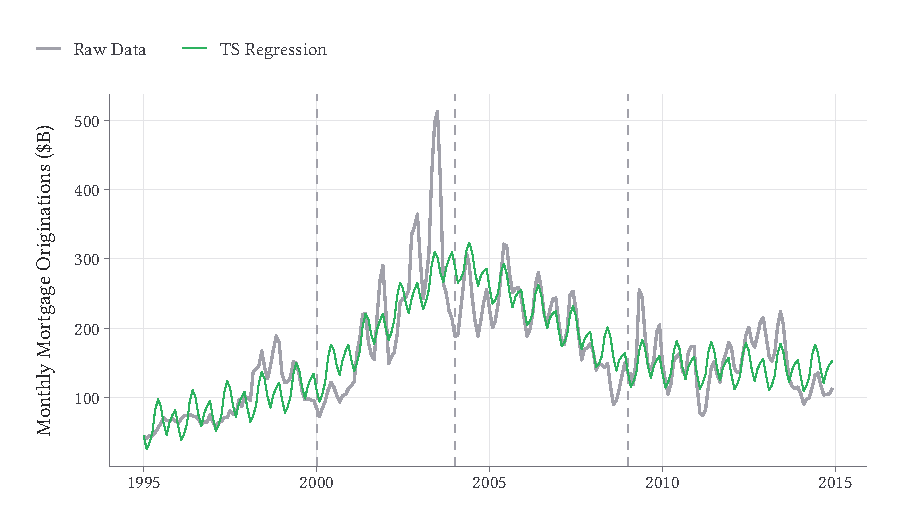
\includegraphics[width = 0.8\textwidth]{figures/raw_data_ts_regression.pdf}
      \end{center}
    \end{figure}

    \begin{figure}[h!]
      \caption{Monthly Mortgage Originations: Raw Data + SES Smoothing}
      \label{fig:raw_ses}

      \vspace*{-2\bigskipamount}
      \begin{center}
        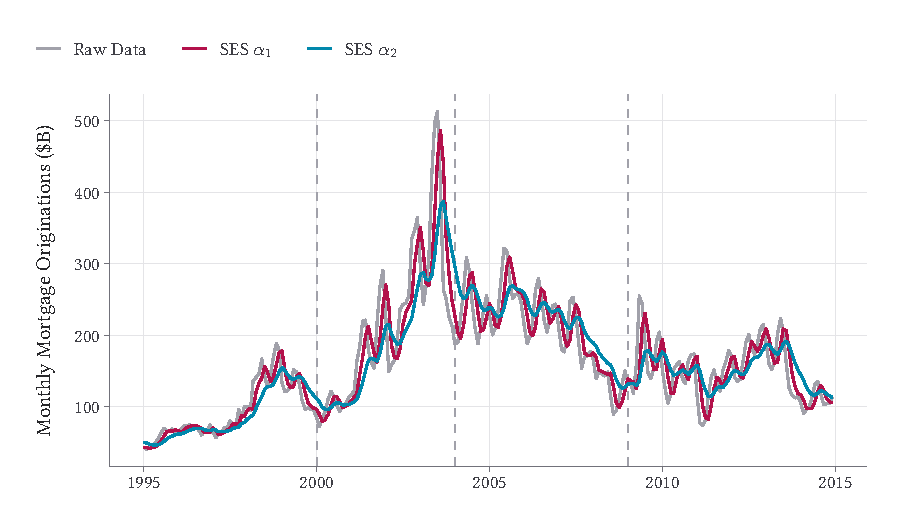
\includegraphics[width = 0.8\textwidth]{figures/raw_data_ses.pdf}
      \end{center}
    \end{figure}

    \newpage
    \begin{codeblock}[{}]
Dependent Var.: m_originations_billion

Constant              -286.0*** (58.9)
date                   0.04*** (0.006)
trend_2                 0.09*** (0.01)
trend_3                -0.21*** (0.02)
trend_4                 0.08*** (0.01)
month = Feb              -20.4. (10.7)
month = Mar               -13.0 (10.5)
month = Apr                0.68 (10.4)
month = May               32.8* (13.5)
month = Jun              47.4** (15.2)
month = Jul               35.8* (15.6)
month = Aug                 9.6 (12.5)
month = Sep                -7.5 (10.7)
month = Oct                 9.9 (11.9)
month = Nov                19.2 (13.3)
month = Dec               24.9. (13.6)
_______________ ______________________
S.E. type             Newey-West (L=0)
---
Signif. codes: 0 '***' 0.001 '**' 0.01 '*' 0.05 '.' 0.1 ' ' 1
    \end{codeblock}

\end{enumerate}
\end{document}
